%=============================================================
%  Auditing Label- and Group-Conditional Coverage for Student Dropout Prediction
%  A Class-Conditional Conformal Prediction Approach
%
%  Rimsha Bibi, M. Umair Shahzad
%  Department of Mathematics, University of Okara, Pakistan
%
%  ------------------------------------------------------------
%  HOW TO COMPILE
%  ------------------------------------------------------------
%  Upload this .tex file and the two Figure4 PNG files together.
%  The existing figures are drawn using pgfplots; the new
%  Figure 4A and Figure 4B are supplied as separate PNG files.
%
%  Overleaf: New Project > Blank Project, paste this whole file
%  into main.tex, and Recompile. Engine: pdfLaTeX.
%  The first compile is slower because the plots are drawn.
%
%  ------------------------------------------------------------
%  JOURNAL FORMATTING
%  ------------------------------------------------------------
%  This file uses the plain `article' class on purpose, so it
%  compiles under a plain article template.
%  Format for a journal only AFTER the journal is chosen:
%  copy everything between \begin{document} and \end{document}
%  into that publisher's template. Nothing in the body below
%  depends on the article class.
%
%  ------------------------------------------------------------
%  BEFORE SUBMISSION
%  ------------------------------------------------------------
%  Confirm every entry in the bibliography against the
%  publisher's own page: volume, issue, year, page range.
%=============================================================
\documentclass[11pt,a4paper]{article}

\usepackage[utf8]{inputenc}
\usepackage[T1]{fontenc}
\usepackage[margin=2.5cm]{geometry}
\usepackage{amsmath,amssymb,amsthm}
\usepackage{booktabs}
\usepackage{graphicx}
\usepackage{caption}
\usepackage{subcaption}
\usepackage{siunitx}
\usepackage{tikz}
\usepackage{pgfplots}
\pgfplotsset{compat=1.18}

% figure palette -- checked for colour-blind separation
\definecolor{fblue}{HTML}{2A78D6}
\definecolor{forange}{HTML}{EB6834}
\definecolor{faqua}{HTML}{1BAF7A}
\definecolor{fgrey}{HTML}{8C8C86}
\definecolor{fdim}{HTML}{9AA4AE}

\usepackage[colorlinks=true,linkcolor=black,citecolor=black,urlcolor=blue]{hyperref}

% --- float placement: keeps figures/tables from leaving large gaps ---
\renewcommand{\topfraction}{0.9}
\renewcommand{\bottomfraction}{0.8}
\renewcommand{\textfraction}{0.07}
\renewcommand{\floatpagefraction}{0.75}
\setcounter{topnumber}{3}
\setcounter{bottomnumber}{2}
\setcounter{totalnumber}{5}

\theoremstyle{plain}
\newtheorem{theorem}{Theorem}
\newtheorem{lemma}[theorem]{Lemma}
\theoremstyle{definition}
\newtheorem{definition}[theorem]{Definition}
\theoremstyle{remark}
\newtheorem{remark}[theorem]{Remark}

\newcommand{\Prob}{\mathbb{P}}
\newcommand{\Ind}{\mathbf{1}}
\newcommand{\Yset}{\mathcal{Y}}
\newcommand{\qhat}{\hat{q}}
\newcommand{\pihat}{\hat{\pi}}

\title{\bfseries Auditing Label- and Group-Conditional Coverage in Three-Class Student Outcome Prediction}

\author{%
Rimsha Bibi \\
\small Department of Mathematics, University of Okara, Okara, Pakistan
\and
M. Umair Shahzad \\
\small Department of Mathematics, University of Okara, Okara, Pakistan
}
\date{}
\title{Supplementary Analyses: Label- and Group-Conditional Student Outcome Coverage}
\author{Rimsha Bibi and Dr. M. Umair Shahzad}
\date{}
\begin{document}
\maketitle
\noindent This supplement reports illustrative single-partition diagnostics and
separately designed ten-partition sensitivity experiments. They are not
substitutes for the manuscript's 100-partition primary analyses.

\section*{S1. Seed-42 point-prediction benchmarks}


Table~\ref{tab:baselines} reports an illustrative seed-42 three-model comparison.
For the 100-partition primary random-forest experiment, mean accuracy was
77.495\% and mean macro-F1 was 0.69267. The other two models were evaluated for conformal coverage over 100
partitions in the main manuscript; their seed-42 point-prediction metrics
in Table~\ref{tab:baselines} are not 100-partition averages.

\begin{table}[htbp]
\centering
\caption{Baseline point classifiers, test partition, seed 42.}
\label{tab:baselines}
\begin{tabular}{lrr}
\toprule
\textbf{Model} & \textbf{Accuracy} & \textbf{Macro-F1} \\
\midrule
Logistic regression            & 76.50\% & 0.6798 \\
Random forest (500 trees)      & 78.53\% & 0.7040 \\
Histogram gradient boosting    & 78.53\% & 0.7259 \\
\bottomrule
\end{tabular}
\end{table}

The baseline classifier scores are specific to the stated 60/20/20
partitions and should not be compared directly with results obtained
using different preprocessing, tuning, or splits.

The aggregate figures conceal a pronounced asymmetry. For the random forest,
per-class recall is 0.946 for \textsf{Graduate}, 0.778 for \textsf{Dropout} and
\textbf{0.352} for \textsf{Enrolled}, with F1 scores of 0.865, 0.795 and 0.452.
The model identifies barely one in three students who remain enrolled, while an
accuracy of 78.53\% presents it as broadly competent. This asymmetry exists
before any uncertainty quantification is applied, and, as we now show,
conformal prediction does not remove it.


\section*{S2. Seed-42 marginal calibration and score distributions}


Calibration on the $n = 885$ held-out students gives
$k = \lceil 886 \times 0.90 \rceil = 798$ and $\qhat = 0.7600$, so a class
enters a student's set whenever the model assigns it probability at least 0.24.
The resulting sets attain an empirical coverage of \textbf{91.19\%} against a
nominal 90\% at an average set size of 1.472 (seed 42; 90.00\% and 1.440
averaged over the ten partitions), and no test student receives an empty set.

Reported at this level---one coverage figure and one average set size---the
method appears to work exactly as advertised. This is the level at which
marginal coverage is ordinarily reported. Over 100 partitions the mean is
90.25\% at an average set size of 1.427; the preceding seed-42
figures are illustrative only.


Figure~\ref{fig:ecdf} shows the mechanism. Mean calibration scores are 0.2498
for \textsf{Graduate}, 0.3396 for \textsf{Dropout} and 0.6477 for
\textsf{Enrolled}: three distributions at different locations, to which one
threshold is applied. The curves cross $\qhat$ at 98.4\%, 88.4\% and 76.1\%
respectively.

\begin{figure}[htbp]
\centering
\begin{tikzpicture}
\begin{axis}[
  width=0.80\textwidth, height=6.0cm,
  xlabel={nonconformity score $s = 1-\hat{\pi}(\mathrm{true\ class})$},
  ylabel={cumulative proportion of class},
  xmin=0, xmax=1.02, ymin=0, ymax=1.04,
  xtick={0,0.2,0.4,0.6,0.8,1.0},
  ytick={0,0.2,0.4,0.6,0.8,1.0},
  grid=major, grid style={fdim!25},
  axis lines=left, tick align=outside,
  legend pos=north west, legend cell align=left,
  legend style={draw=none, fill=white, fill opacity=0.9, text opacity=1, font=\footnotesize},
  label style={font=\small}, tick label style={font=\footnotesize},
]
\addplot[const plot, fblue, thick] coordinates {(0,0) (0.0040,0.0035) (0.0060,0.0106) (0.0100,0.0211) (0.0120,0.0282) (0.0140,0.0387) (0.0160,0.0458) (0.0180,0.0563) (0.0180,0.0669) (0.0180,0.0739) (0.0240,0.0845) (0.0260,0.0915) (0.0260,0.1021) (0.0280,0.1127) (0.0280,0.1197) (0.0380,0.1303) (0.0400,0.1373) (0.0460,0.1479) (0.0520,0.1585) (0.0560,0.1655) (0.0620,0.1761) (0.0640,0.1831) (0.0700,0.1937) (0.0700,0.2042) (0.0760,0.2113) (0.0780,0.2218) (0.0800,0.2289) (0.0840,0.2394) (0.0880,0.2500) (0.0900,0.2570) (0.0980,0.2676) (0.1020,0.2746) (0.1060,0.2852) (0.1140,0.2958) (0.1200,0.3028) (0.1220,0.3134) (0.1260,0.3204) (0.1380,0.3310) (0.1480,0.3415) (0.1540,0.3486) (0.1580,0.3592) (0.1600,0.3662) (0.1660,0.3768) (0.1760,0.3873) (0.1800,0.3944) (0.1900,0.4049) (0.1940,0.4120) (0.2000,0.4225) (0.2080,0.4331) (0.2140,0.4401) (0.2240,0.4507) (0.2240,0.4577) (0.2480,0.4683) (0.2680,0.4789) (0.2680,0.4859) (0.2780,0.4965) (0.2820,0.5035) (0.2940,0.5141) (0.3000,0.5211) (0.3120,0.5317) (0.3400,0.5423) (0.3440,0.5493) (0.3460,0.5599) (0.3560,0.5669) (0.3600,0.5775) (0.3720,0.5880) (0.3800,0.5951) (0.3840,0.6056) (0.3920,0.6127) (0.4120,0.6232) (0.4180,0.6338) (0.4240,0.6408) (0.4360,0.6514) (0.4420,0.6585) (0.4580,0.6690) (0.4860,0.6796) (0.4940,0.6866) (0.5040,0.6972) (0.5060,0.7042) (0.5180,0.7148) (0.5260,0.7254) (0.5380,0.7324) (0.5500,0.7430) (0.5580,0.7500) (0.5660,0.7606) (0.5720,0.7711) (0.5840,0.7782) (0.5980,0.7887) (0.6000,0.7958) (0.6100,0.8063) (0.6280,0.8169) (0.6360,0.8239) (0.6540,0.8345) (0.6620,0.8415) (0.7020,0.8521) (0.7220,0.8627) (0.7400,0.8697) (0.7580,0.8803) (0.7620,0.8873) (0.7740,0.8979) (0.8140,0.9085) (0.8240,0.9155) (0.8340,0.9261) (0.8360,0.9331) (0.8600,0.9437) (0.8740,0.9542) (0.8760,0.9613) (0.9400,0.9718) (0.9520,0.9789) (0.9700,0.9894) (0.9860,1.0000) (1.02,1)};
\addlegendentry{Dropout}
\addplot[const plot, forange, thick] coordinates {(0,0) (0.3700,0.0063) (0.4080,0.0126) (0.4080,0.0189) (0.4380,0.0314) (0.4480,0.0377) (0.4500,0.0503) (0.4520,0.0566) (0.4800,0.0692) (0.4840,0.0755) (0.4900,0.0881) (0.4920,0.0943) (0.4940,0.1006) (0.5020,0.1132) (0.5080,0.1195) (0.5100,0.1321) (0.5120,0.1384) (0.5180,0.1509) (0.5220,0.1572) (0.5260,0.1698) (0.5260,0.1761) (0.5280,0.1824) (0.5320,0.1950) (0.5320,0.2013) (0.5360,0.2138) (0.5380,0.2201) (0.5460,0.2327) (0.5480,0.2390) (0.5520,0.2516) (0.5520,0.2579) (0.5560,0.2704) (0.5560,0.2767) (0.5580,0.2830) (0.5600,0.2956) (0.5620,0.3019) (0.5640,0.3145) (0.5640,0.3208) (0.5680,0.3333) (0.5700,0.3396) (0.5700,0.3522) (0.5740,0.3585) (0.5760,0.3648) (0.5880,0.3774) (0.5900,0.3836) (0.5940,0.3962) (0.5980,0.4025) (0.6000,0.4151) (0.6020,0.4214) (0.6120,0.4340) (0.6120,0.4403) (0.6280,0.4528) (0.6280,0.4591) (0.6300,0.4654) (0.6340,0.4780) (0.6400,0.4843) (0.6400,0.4969) (0.6400,0.5031) (0.6440,0.5157) (0.6460,0.5220) (0.6540,0.5346) (0.6600,0.5409) (0.6640,0.5472) (0.6780,0.5597) (0.6800,0.5660) (0.6880,0.5786) (0.6880,0.5849) (0.6960,0.5975) (0.7040,0.6038) (0.7040,0.6164) (0.7040,0.6226) (0.7160,0.6352) (0.7180,0.6415) (0.7180,0.6478) (0.7220,0.6604) (0.7240,0.6667) (0.7340,0.6792) (0.7340,0.6855) (0.7360,0.6981) (0.7380,0.7044) (0.7440,0.7170) (0.7440,0.7233) (0.7460,0.7296) (0.7480,0.7421) (0.7540,0.7484) (0.7580,0.7610) (0.7640,0.7673) (0.7680,0.7799) (0.7740,0.7862) (0.7800,0.7987) (0.7940,0.8050) (0.7980,0.8176) (0.8040,0.8239) (0.8040,0.8302) (0.8140,0.8428) (0.8200,0.8491) (0.8280,0.8616) (0.8320,0.8679) (0.8440,0.8805) (0.8480,0.8868) (0.8540,0.8994) (0.8680,0.9057) (0.8740,0.9119) (0.8860,0.9245) (0.8980,0.9308) (0.9080,0.9434) (0.9100,0.9497) (0.9260,0.9623) (0.9300,0.9686) (0.9440,0.9811) (0.9540,0.9874) (0.9940,1.0000) (1.02,1)};
\addlegendentry{Enrolled}
\addplot[const plot, faqua, thick] coordinates {(0,0) (0.0100,0.0023) (0.0180,0.0113) (0.0240,0.0204) (0.0280,0.0294) (0.0320,0.0385) (0.0380,0.0475) (0.0380,0.0566) (0.0440,0.0656) (0.0460,0.0747) (0.0480,0.0837) (0.0540,0.0928) (0.0620,0.1018) (0.0640,0.1109) (0.0680,0.1199) (0.0680,0.1290) (0.0720,0.1380) (0.0780,0.1471) (0.0800,0.1561) (0.0840,0.1652) (0.0880,0.1742) (0.0880,0.1833) (0.0900,0.1923) (0.0940,0.2036) (0.0980,0.2127) (0.1000,0.2217) (0.1020,0.2308) (0.1040,0.2398) (0.1060,0.2489) (0.1120,0.2579) (0.1160,0.2670) (0.1200,0.2760) (0.1240,0.2851) (0.1280,0.2941) (0.1320,0.3032) (0.1360,0.3122) (0.1380,0.3213) (0.1420,0.3303) (0.1440,0.3394) (0.1460,0.3484) (0.1480,0.3575) (0.1540,0.3665) (0.1580,0.3756) (0.1660,0.3846) (0.1680,0.3937) (0.1720,0.4050) (0.1760,0.4140) (0.1780,0.4231) (0.1860,0.4321) (0.1880,0.4412) (0.1900,0.4502) (0.1940,0.4593) (0.2020,0.4683) (0.2040,0.4774) (0.2080,0.4864) (0.2140,0.4955) (0.2160,0.5045) (0.2180,0.5136) (0.2220,0.5226) (0.2280,0.5317) (0.2320,0.5407) (0.2420,0.5498) (0.2440,0.5588) (0.2500,0.5679) (0.2580,0.5769) (0.2660,0.5860) (0.2720,0.5950) (0.2820,0.6063) (0.2860,0.6154) (0.2940,0.6244) (0.2960,0.6335) (0.2980,0.6425) (0.3060,0.6516) (0.3140,0.6606) (0.3180,0.6697) (0.3260,0.6787) (0.3300,0.6878) (0.3380,0.6968) (0.3400,0.7059) (0.3520,0.7149) (0.3580,0.7240) (0.3660,0.7330) (0.3700,0.7421) (0.3740,0.7511) (0.3900,0.7602) (0.3960,0.7692) (0.4040,0.7783) (0.4140,0.7873) (0.4240,0.7964) (0.4380,0.8077) (0.4480,0.8167) (0.4580,0.8258) (0.4700,0.8348) (0.4760,0.8439) (0.4840,0.8529) (0.5020,0.8620) (0.5100,0.8710) (0.5180,0.8801) (0.5320,0.8891) (0.5320,0.8982) (0.5460,0.9072) (0.5500,0.9163) (0.5600,0.9253) (0.5920,0.9344) (0.6000,0.9434) (0.6240,0.9525) (0.6440,0.9615) (0.6580,0.9706) (0.7200,0.9796) (0.7760,0.9887) (0.8820,1.0000) (1.02,1)};
\addlegendentry{Graduate}
\addplot[black, dashed, thin] coordinates {(0.7600,0) (0.7600,1.04)};
\addplot[black, dotted, thin, forget plot] coordinates {(0,0.90) (1.02,0.90)};
\addplot[only marks, mark=*, mark size=1.8pt, fblue, forget plot] coordinates {(0.7600,0.8838)};
\node[anchor=west, font=\scriptsize\bfseries, fblue, fill=white, fill opacity=0.85, text opacity=1, inner sep=1pt] at (axis cs:0.7800,0.8838) {88.4\%};
\addplot[only marks, mark=*, mark size=1.8pt, forange, forget plot] coordinates {(0.7600,0.7610)};
\node[anchor=west, font=\scriptsize\bfseries, forange, fill=white, fill opacity=0.85, text opacity=1, inner sep=1pt] at (axis cs:0.7800,0.7610) {76.1\%};
\addplot[only marks, mark=*, mark size=1.8pt, faqua, forget plot] coordinates {(0.7600,0.9842)};
\node[anchor=west, font=\scriptsize\bfseries, faqua, fill=white, fill opacity=0.85, text opacity=1, inner sep=1pt] at (axis cs:0.7800,0.9842) {98.4\%};
\node[anchor=east, font=\scriptsize] at (axis cs:0.7400,0.06) {global $\hat{q}=0.76$};
\node[anchor=west, font=\scriptsize] at (axis cs:0.35,0.935) {target 0.90};
\end{axis}
\end{tikzpicture}
\caption{Cumulative distribution of the nonconformity score
$s = 1-\hat{\pi}(\text{true class})$ on the test partition, by realised outcome.
Where each class's curve crosses the global threshold $\hat q = 0.76$ is that
class's coverage. Random forest (500 trees), stratified 60/20/20 split,
$\alpha = 0.10$, LAC score, seed 42.}
\label{fig:ecdf}
\end{figure}
\section*{S3. Seed-42 Mondrian thresholds and set sizes}
Calibrating within classes gives $\qhat_{\textsf{Dropout}} = 0.830$,
$\qhat_{\textsf{Enrolled}} = 0.850$ and $\qhat_{\textsf{Graduate}} = 0.528$ on
seed 42, against the global $\qhat = 0.760$. The ordering makes the mechanism
explicit: \textsf{Enrolled} required a threshold well above the global value and
was denied it, while \textsf{Graduate} required one well below and received far
more than it needed.


\begin{figure}[htbp]
\centering
\begin{tikzpicture}
\begin{axis}[
  width=0.72\textwidth, height=5.6cm,
  ybar, bar width=17pt,
  xlabel={prediction-set size $|C(x)|$},
  ylabel={\% of test students},
  symbolic x coords={1,2,3}, xtick=data,
  ymin=0, ymax=68,
  grid=major, grid style={fdim!25},
  axis lines=left, tick align=outside,
  legend style={draw=none, at={(0.98,0.97)}, anchor=north east, font=\footnotesize},
  legend cell align=left,
  label style={font=\small}, tick label style={font=\footnotesize},
  nodes near coords, nodes near coords style={font=\scriptsize,
      /pgf/number format/fixed, /pgf/number format/precision=1,
      /pgf/number format/fixed zerofill},
]
\addplot[fill=fgrey, draw=fgrey] coordinates {(1,59.32) (2,34.12) (3,6.55)};
\addlegendentry{split CP}
\addplot[fill=fblue, draw=fblue] coordinates {(1,44.18) (2,51.19) (3,4.63)};
\addlegendentry{Mondrian CP}
\end{axis}
\end{tikzpicture}
\caption{Distribution of prediction-set size under split and Mondrian conformal
prediction. Random forest (500 trees), $\alpha = 0.10$, LAC score, seed 42.}
\label{fig:setsize}
\end{figure}
\section*{S4. Deterministic cumulative-score sensitivity (ten seeds)}
A separate exploratory ten-partition analysis used the deterministic
candidate score $A_{\mathrm{cum}}(x,c)=\sum_{j:\,\mathrm{rank}(j)\le
\mathrm{rank}(c)}\hat\pi(j\mid x)$, with labels admitted when
$A_{\mathrm{cum}}(x,c)\le\hat q$ (including the boundary). It gave overall,
\textsf{Dropout}, \textsf{Enrolled} and \textsf{Graduate} coverages of
90.47\%, 83.17\%, 84.97\% and 97.15\%, respectively, with mean set size
1.813 and 18 empty sets per test partition on average. This convention can
return the empty set when even the largest class probability exceeds the
calibrated threshold. It is \emph{not} the same set construction as the
threshold-crossing-prefix APS convention that includes the class crossing the
threshold. Accordingly these exploratory results are reported only to make
implementation sensitivity transparent; no coverage claim for canonical
nonrandomized APS is based on them. In particular, score definition,
tie-breaking, threshold inclusion and test-time randomization must be matched
when comparing APS variants.


\section*{S5. Training-only RF tuning (ten seeds)}


On the original ten partitions, we used 3-fold stratified cross-validation
\emph{within the 60\% training subset} to select hyperparameters by macro-F1,
with ten random search draws per seed over 200--500 trees, max depths
\{None, 10, 20, 30\}, split sizes \{2,5,10\}, leaf sizes \{1,2,4\},
and feature subsampling \{sqrt, log2\}. Calibration and test samples were
held out from both training and tuning. The default model had 500 trees.

\begin{table}[htbp]
\centering\small
\caption{Training-only tuned RF versus default RF; ten-partition mean.
Accuracy, macro-F1, and coverage are percentages.}
\label{tab:tuned}
\begin{tabular}{lrrrrr}
\toprule Model & Accuracy & Macro-F1 & Split Enrolled & Mondrian Enrolled & Mondrian size\\
\midrule
Default RF & 76.350 & 68.055 & 73.145 & 89.937 & 1.603\\
Tuned RF & 76.158 & 67.464 & 72.830 & 90.189 & 1.611\\
\bottomrule
\end{tabular}
\end{table}

The mean paired tuned-minus-default differences across these ten overlapping
partitions were $-0.192$ percentage points for accuracy and $-0.591$ for
macro-F1, with partition-based $t$-intervals $[-0.617,0.232]$ and
$[-1.121,-0.061]$, respectively. These intervals measure variability
across resampling seeds on the \emph{same} cohort; they must not be
interpreted as inference from ten independent student populations. This
sensitivity experiment provides no evidence that the tested tuning process
resolves global split-CP undercoverage for \textsf{Enrolled}.


\section*{S6. Seed-42 singleton selection and alpha sweep}
A singleton set is a possible selection rule, not a conditional risk
certificate. At seed 42, Mondrian CP produced 391 singletons (44.18\% of
885 students), with 90.79\% \emph{delivered-label} accuracy and 92.07\%
top-1 accuracy on those same students. Ranking all 885 students by maximum
predicted class probability and choosing the top 391 gave 94.12\% top-1
accuracy. The distinction matters because the sole candidate label in a
Mondrian singleton need not be the highest-probability class.


A seed-42 sensitivity sweep across $\alpha=0.02,0.03,\ldots,0.40$
(39 values) gives the matched maximum-probability baseline accuracy at least
as high as Mondrian \emph{delivered} singleton accuracy at every value
(Figure~\ref{fig:selection-sweep}a). At $\alpha=0.10$, delivered, singleton
subset top-1, and matched maximum-probability accuracy are 90.79\%,
92.07\%, and 94.12\%, respectively. At $\alpha=0.20$ the delivered
accuracy drops to 77.50\% while the selected fraction is 77.85\%, and
12 test points receive empty sets. The singleton fraction is
\emph{non-monotone}: it peaks at 84.86\% near $\alpha=0.25$ and falls
to 72.20\% at $\alpha=0.40$, where 241 of 885 test students receive
empty sets (Figure~\ref{fig:selection-sweep}b). Empty sets are not
considered automatic decisions. This sweep concerns selective performance,
not a guarantee of conditional accuracy among selected students.

\begin{figure}[htbp]
\centering
\begin{subfigure}{\textwidth}
\centering
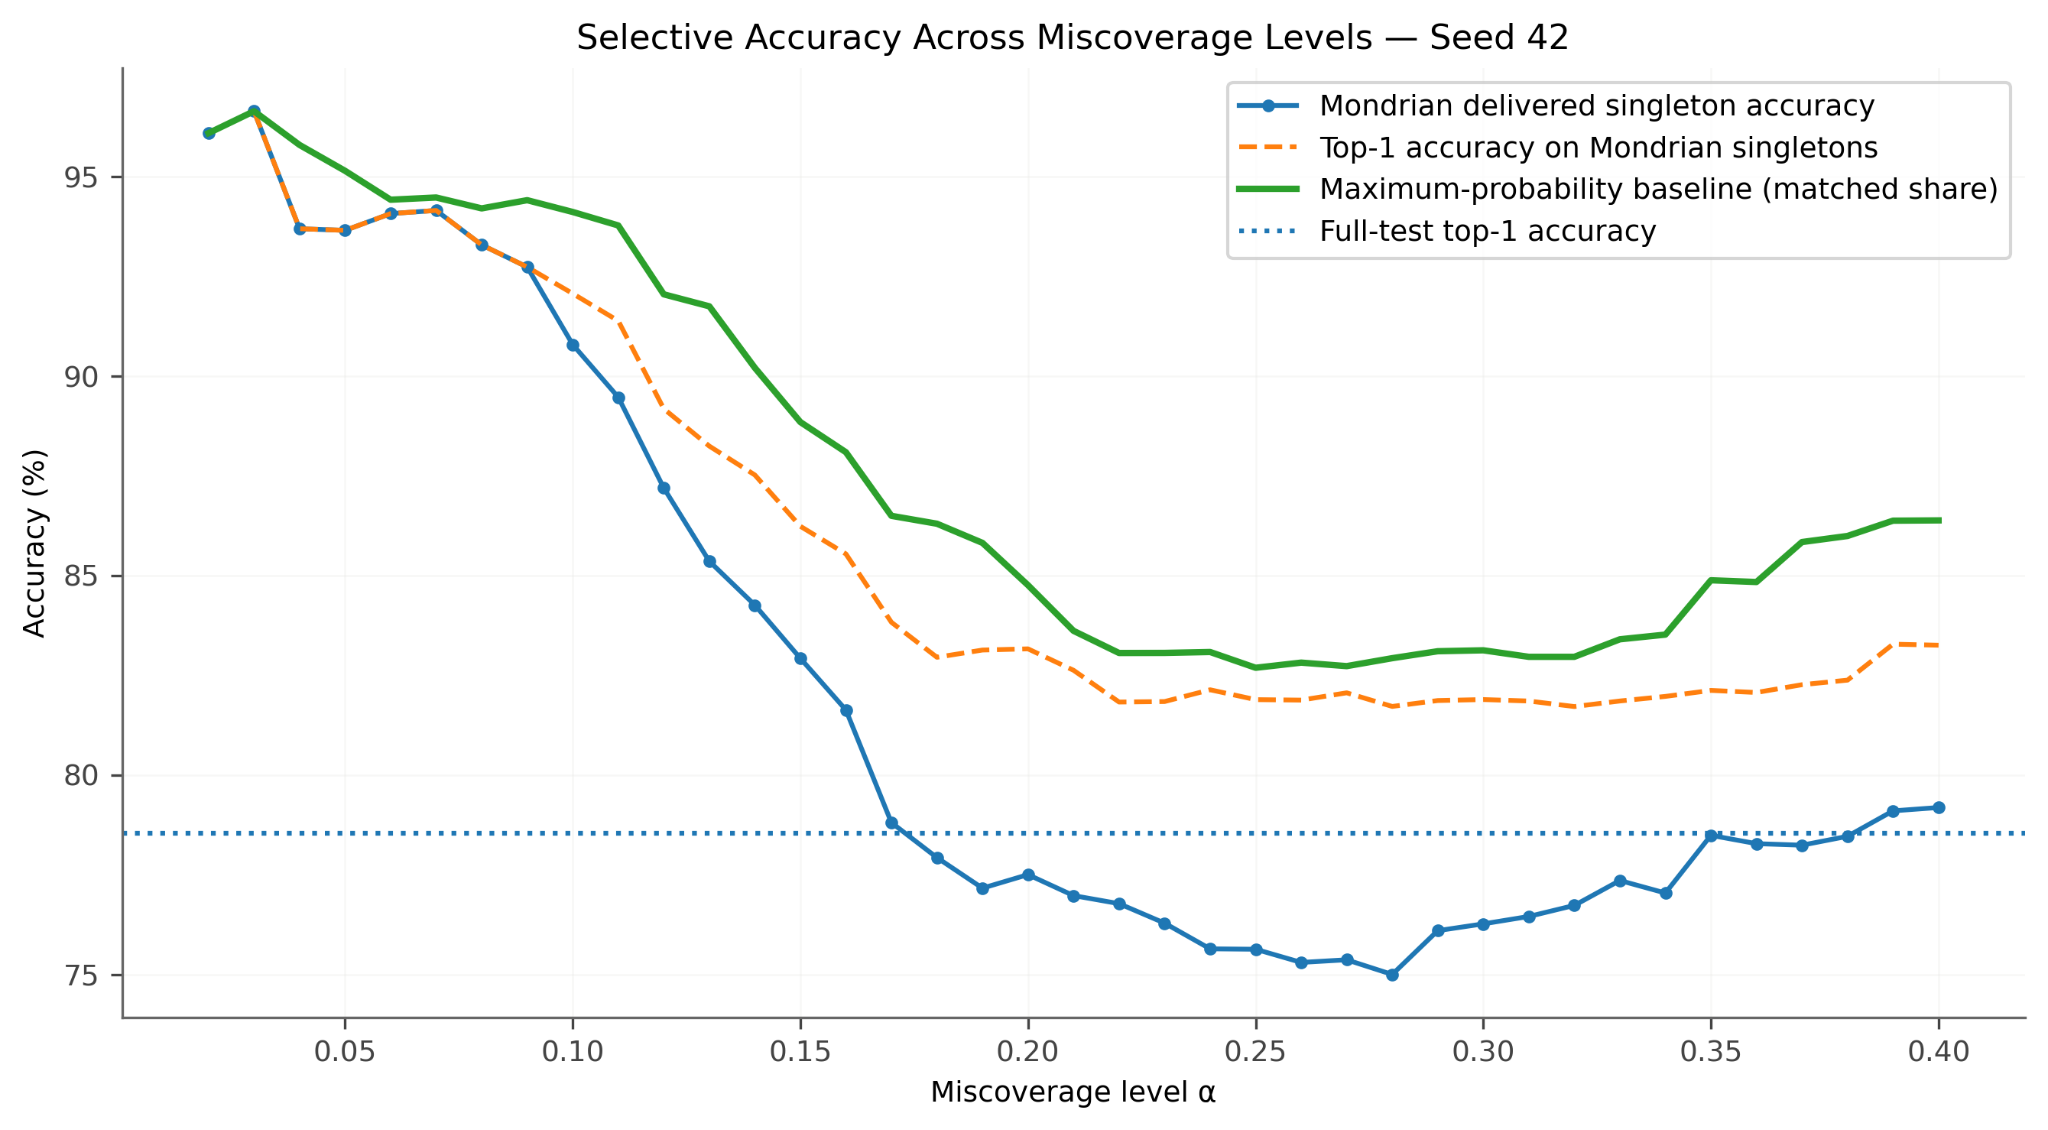
\includegraphics[width=0.97\linewidth]{Figure4A_accuracy.png}
\caption{Delivered singleton accuracy, top-1 accuracy on the same singleton subset, and top-1 accuracy of a maximum-probability baseline selecting the same number of students; dotted line shows unconditional test top-1 accuracy.}
\end{subfigure}
\vspace{0.6em}
\begin{subfigure}{\textwidth}
\centering
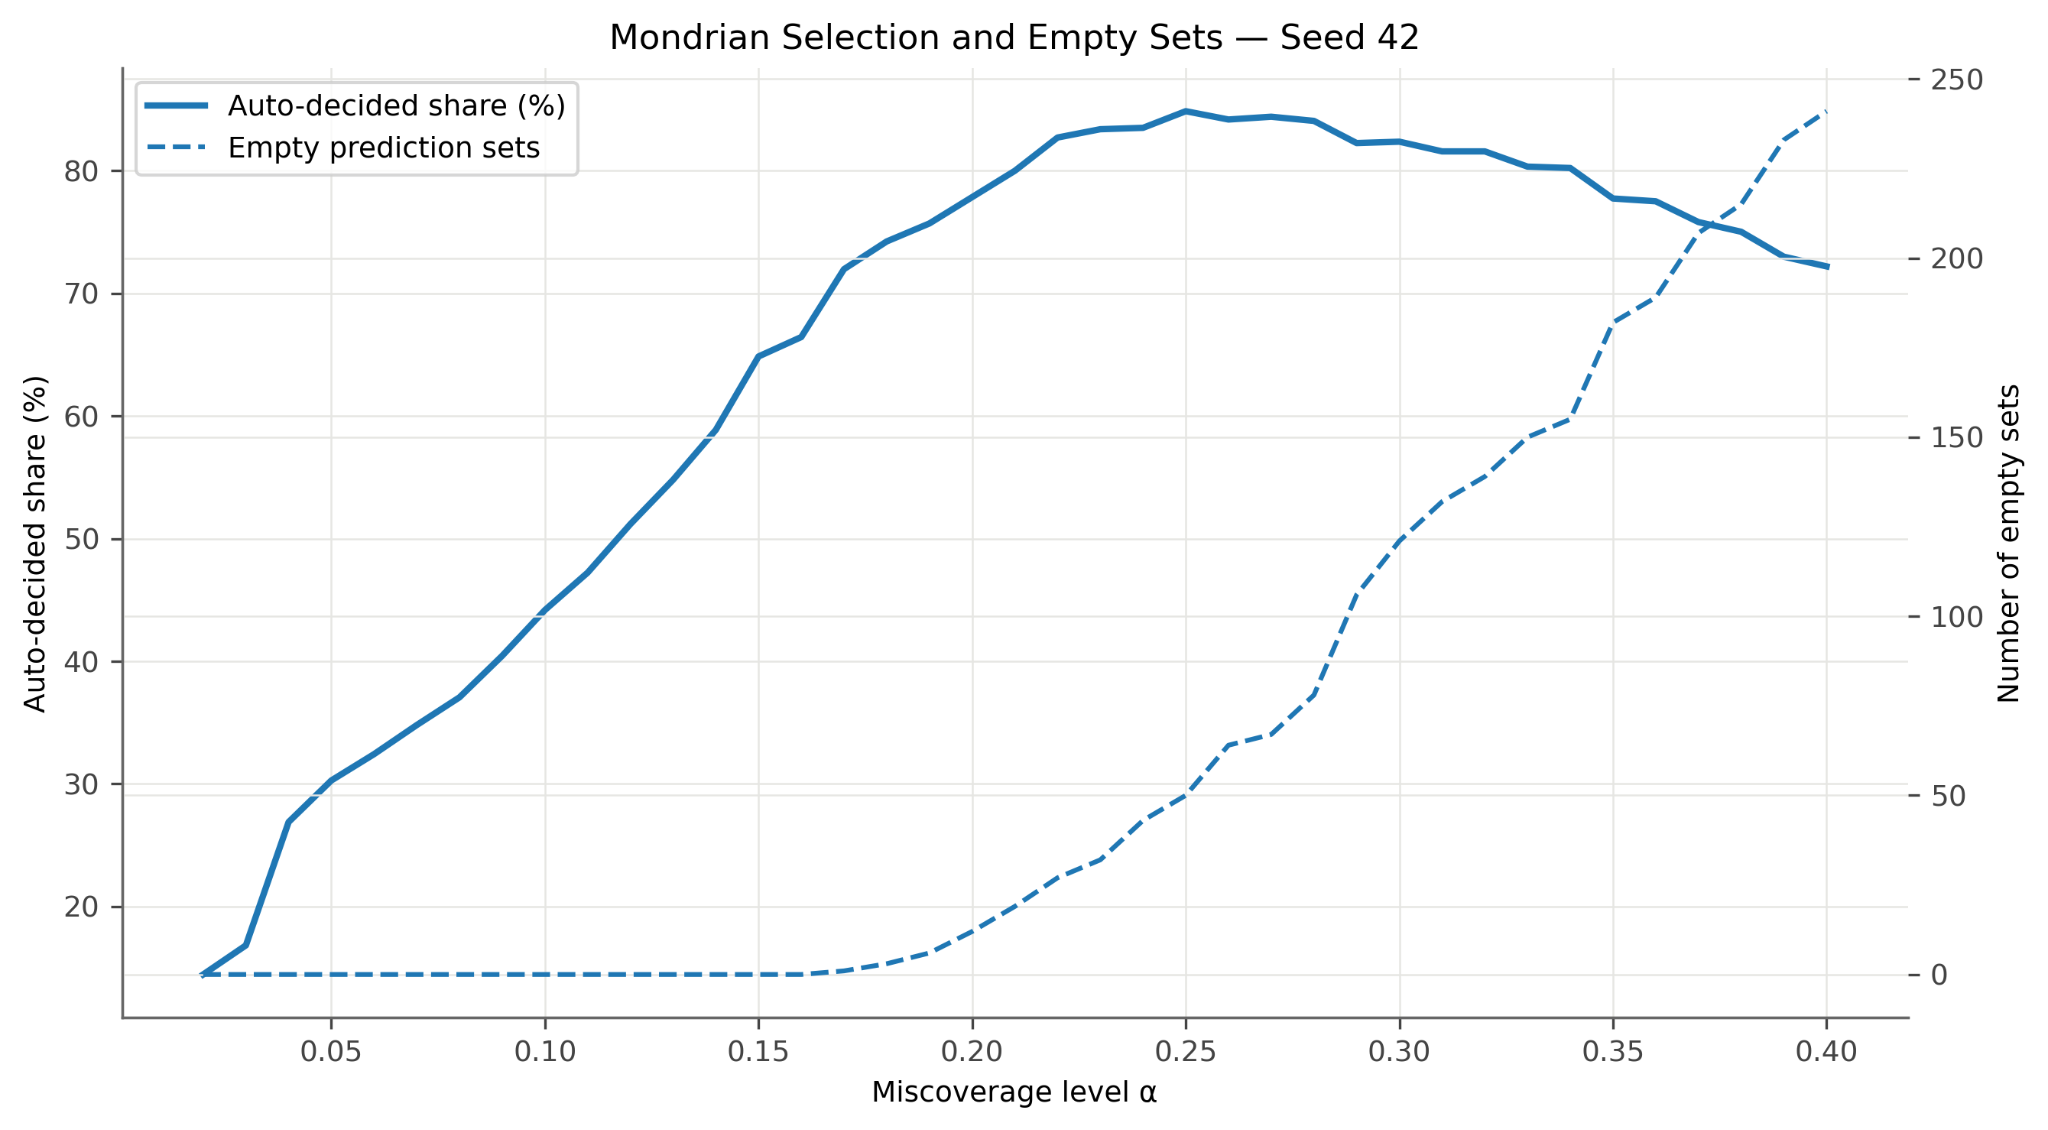
\includegraphics[width=0.97\linewidth]{Figure4B_selection.png}
\caption{Fraction with exactly one candidate label (left axis) and number with no candidate label (right axis).}
\end{subfigure}
\caption{Seed-42 Mondrian conformal sensitivity analysis on 885 test
students across 39 miscoverage levels, $\alpha=0.02$--$0.40$.
``Delivered'' accuracy is accuracy of the unique label in the singleton
set; ``top-1'' is accuracy of the classifier's most probable class.
Selection sizes for maximum-probability ranking match the Mondrian singleton
count at each $\alpha$. Empty sets are excluded from both the singleton
numerator and the auto-decision count.}
\label{fig:selection-sweep}
\end{figure}


\end{document}